\documentclass[11pt]{report}
\usepackage[utf8]{inputenc}
\usepackage[a4paper, margin=1in]{geometry}
\usepackage{graphicx, color}
\usepackage{booktabs}
\usepackage[toc,page]{appendix}
\usepackage{pdfpages}
\usepackage{multicol}
\usepackage{changepage}
\usepackage{float}
\usepackage{multirow}
\usepackage{amsmath}
\usepackage[encoding,filenameencoding=utf8]{grffile}
\usepackage{subcaption}
\usepackage{csquotes}
\usepackage{hyperref, bookmark}

\setlength{\columnseprule}{0.5pt}
\def\columnseprulecolor{\color{black}}


% Package de algoritmos
\usepackage[portuguese,ruled,lined]{algorithm2e}

% Portuguese Encoding 
\usepackage[portuguese]{babel}
\usepackage[T1]{fontenc}

% import Java
\usepackage{listings} 

% Header
\usepackage{fancyhdr}
\pagestyle{fancy}
	\fancyhf{}
		\lhead{LEIC - ISEL}
    \rhead{Lógica e Computação}

% Footer
\renewcommand{\headrulewidth}{1pt}
\renewcommand{\footrulewidth}{1pt}
\fancyfoot[CE,CO]{\thepage}


%%%%%%%%%%%%%%%%%%%%%%%%%%%%%%%%%%%%%%%%% CHANGES %%%%%%%%%%%%%%%%%%%%%%%%%%%%%%%%%


% Redefine the plain page style
\fancypagestyle{plain}{
\pagestyle{fancy}
  \fancyhf{}
	\lhead{LEIC - ISEL}
	\rhead{Computação Informática}
	\renewcommand{\headrulewidth}{1pt}
	\renewcommand{\footrulewidth}{1pt}
\fancyfoot[CE,CO]{\thepage}
}

%%%%%%%%%%%%%%%%%%%%%%%%%%%%%%%%%%%%%%%%% CHANGES %%%%%%%%%%%%%%%%%%%%%%%%%%%%%%%%%

% Titulo e informação de capa
\title{Segunda fase do trabalho Prático}
\date{Dezembro 2019}

% Define Chapter heading
\makeatletter
\def\@makechapterhead#1{%
  \vspace*{20\p@}%                                 % Insert 50pt (vertical) space
  {\parindent \z@ \raggedright \normalfont         % No paragraph indent, ragged right
%    \interlinepenalty\@M                           % Penalty
    \huge \bfseries #1\par\nobreak                 % Huge, bold chapter title
    \vskip 10\p@                                   % Insert 40pt (vertical) space
  }}
  
  %%%%%%%%%%%%%%%%%%%%%%%%%%%%%%%%%%%%%%%%% CHANGES %%%%%%%%%%%%%%%%%%%%%%%%%%%%%%%%%

\makeatother

%Custom commands

\renewcommand\appendixpagename{Anexos}
\renewcommand\appendixname{Anexo}
\renewcommand\appendixtocname{Anexos}

\newenvironment{subs}
  {\adjustwidth{2.5em}{0pt}}
  {\endadjustwidth}


% Retira a indentação ao início dos parágrafos 
\setlength{\parindent}{0em}
\newcommand{\blank}[1]{\hspace*{#1}\linebreak[0]}

% Section and Subsection spacing:
\usepackage{titlesec}
\usepackage{lipsum}



%%%%%%%%%%%%%%%%%%%%%%%%%%%%%%%%%%	DOCUMENT BEGINS	%%%%%%%%%%%%%%%%%%%%%%%%%%%%%%%%%%%%%

\begin{document}

%%%%%%%%%%%%%%%%%%%%%%%%%%%%%%%%%%%%%%%%%%%%%%%%%%%%%%%%%%%%%%%%%%%%%%%%%%%%%%%%%%%%%%%%%
%										COVER											%
%%%%%%%%%%%%%%%%%%%%%%%%%%%%%%%%%%%%%%%%%%%%%%%%%%%%%%%%%%%%%%%%%%%%%%%%%%%%%%%%%%%%%%%%%

\begin{titlepage} 

\newcommand{\HRule}{\rule{\linewidth}{0.5mm}} % Defines a new command for the horizontal lines, change thickness here

%----------------------------------------------------------------------------------------
%	LOGO SECTION
%----------------------------------------------------------------------------------------


\includegraphics[width=130pt, keepaspectratio=true]{img/logo_isel}\\[1cm] % Include a department/university logo - this will require the graphicx package
\center % Center everything on the page
 
%----------------------------------------------------------------------------------------
%	HEADING SECTIONS
%----------------------------------------------------------------------------------------

\textsc{\LARGE INSTITUTO SUPERIOR DE ENGENHARIA DE LISBOA}\\[1.5cm] % Name of your university/college
\vskip 40pt
\textsc{\Large LÓGICA E COMPUTAÇÃO}\\[0.5cm] % Major heading such as course name
\textsc{\large LICENCIATURA ENGENHARIA INFORMÁTICA E COMPUTADORES}\\[0.5cm] % Minor heading such as course title
\vskip 40pt

%----------------------------------------------------------------------------------------
%	TITLE SECTION
%----------------------------------------------------------------------------------------

\HRule \\[0.4cm]
{ \LARGE \bfseries TRABALHO PRÁTICO }\\[0.4cm]
{ \huge \bfseries Fase 2}\\[0.4cm] % Title of your document
\HRule \\[1.5cm]
 
%----------------------------------------------------------------------------------------
%	AUTHOR SECTION
%----------------------------------------------------------------------------------------
\vskip 70pt
\begin{minipage}{0.4\textwidth}
\begin{flushleft} \large
\emph{Autor:}\\
43552 - Samuel \textsc{Costa}\\
\end{flushleft}
\end{minipage}
~
\begin{minipage}{0.4\textwidth}
\begin{flushright} \large
\emph{Docente:} \\
Walter \textsc{VIEIRA}\\
\end{flushright}
\end{minipage}\\[3cm]

%----------------------------------------------------------------------------------------
%	DATE SECTION
%----------------------------------------------------------------------------------------

{\large 22 de Dezembro de 2019}\\[3cm] % Date, change the \today to a set date if you want to be precise

%----------------------------------------------------------------------------------------

\vfill % Fill the rest of the page with whitespace

\end{titlepage}


\renewcommand\thesection{\arabic{section}}

\pdfbookmark{\contentsname}{toc}
\tableofcontents


\newpage


\section*{Introdução}
Este relatório, referente à Segunda fase do trabalho prático, foi elaborado no 
âmbito da unidade curricular de Lógica e Computação e acompanha a realização de um programa prolog que realiza pesquisa em profundidade para determinação do caminho entre dois pontos de um labirinto. A realização do trabalho seguiu de perto o guião fornecido pelo docente, pelo que a sua descrição também adere a essa sequência.
\newpage

\section{Caracterização e modelação do problema}
Foi proposta a realização de um programa Prolog para determinação de caminhos dentro de um labirinto.
Identificou-se um algoritmo apropriado, designadamente o algoritmo de pesquisa em profundidade com Hill Climbing para labirintos que não incluam caminhos "muito recortados" e o algoritmo de pesquisa em profundidade pura para os outros labirintos.\\
A implementação do algoritmo exigiu que se formalizasse a representação de uma casa do labirinto, um estado - que corresponde a uma movimentação no labirinto - bem como as regras de progressão de estado.\\
O labirinto é caracterizado por uma lista de saídas.\\
As saídas são representadas pelo predicado saida(X,Y,D), em que X e Y são coordenadas no labirinto e D é uma das quatro direcções (d - direita, e - esquerda, c - cima, b - baixo).\\
Uma casa no labirinto é caracterizada pela sua abcissa e ordenada. Na representação visual do labirinto, a origem do referencial é o seu canto superior esquerdo. Assim, uma casa pode ser modelada em prolog pelo predicado casa(X,Y) (ex: casa(1,2)).\\
O estado corresponde a uma movimentação entre casas adjacentes, desde uma casa de origem para uma casa de destino e é representado pelo predicado estado(CasaOrigem,CasaDestino).\\
Como dissemos, progride-se no labirinto entre casas adjacentes, isto é, é possível progredir de uma casa para outra, se houver uma saida dessa casa numa das quatro direcções (esquerda, direita, baixo, cima), ou se houver uma saída de uma casa numa das quatro direcções para a casa que estivermos a considerar.\\


\section{Ponto 1}
	Definiu-se o predicado liga(Casa1,Casa2), que sucede quando há saída da Casa1 movimentando-se para cima, ou seja, se a abcissa das duas casas é a mesma e se a ordenada da segunda casa for igual à primeira mais um. Também sucede, se da Casa 2 for possivel movimentar-se para baixo e a Casa1 estiver em baixo da Casa2. Sucede ainda em outros dois caso, se da Casa1 for possível movimentar-se para a direita e for a Casa2 que estiver nessa direcção, ou se da Casa2 for possível movimentar-se para a esquerda e a Casa1 estiver nesse lugar. O predicado ligaBid(X,Y,D), sucede com D igual a 1 se o predicado liga(X,Y) suceder. Uma vez que a relação é reflexiva, o predicado também sucede se o predicado liga(Y,X) suceder. Desta forma, o predicado "liga" não precisa de ser exaustivamente definido para as quatro direções de ligação possíveis, bastando apenas defini-lo para a movimentação para cima e para a direita.
\section{Ponto 2}
	O predicado "podeJuntar" foi definido à custa de um predicado auxiliar "podeJuntar1", que sucede, produzindo uma nova lista com as casas visitadas, se o estado presente não se encontrar na lista de visitados.

\section{Ponto 3}
	Foi definido o predicado "novoEstado" que sucede produzindo um estado sucessor do actual e alterando a distância percorrida. Se a distância percorrida exceder a distância máxima o predicado falha.

\section{Ponto 4}
	Foi definido o predicado "novoEstadoHC" que sucede produzindo um estado sucessor do actual e a distância em linha recta entre a casa inicial do novo estado e a casa de destino.

\section{Ponto 5}
	Foi definido o predicado "resolverLabirinto" que utiliza o predicado auxiliar "pesqProf". Este utiliza o predicado novoEstado para gerar estados sucessores do actual e acrescentá-los à lista de estados que integram o caminho. Este predicado é chamado recursivamente até que a casa actual do estado seja igual à final. Como este algoritmo se destina a ser chamado no contexto de um sistema de prolog que recebe o estado sob a forma e(Casa1,Casa2), foi definido o predicado "transformar" que muda o formato de representação do estado de estado(Casa1,Casa2) para o formato referido.

\section{Ponto 6}
	Foi definido o predicado "resolver" que, por unificação, obtem a distância máxima a partir da base de dados e chama o predicado resolver labirinto, fazendo reflecir na base de dados a distância percorrida no final da execução do algoritmo. Na figura abaixo se apresenta uma captura de ecrã do sistema em funcionamento, utilizando o algoritmo de pesquisa HC desenvolvido.
	
\begin{figure}[!htb]
	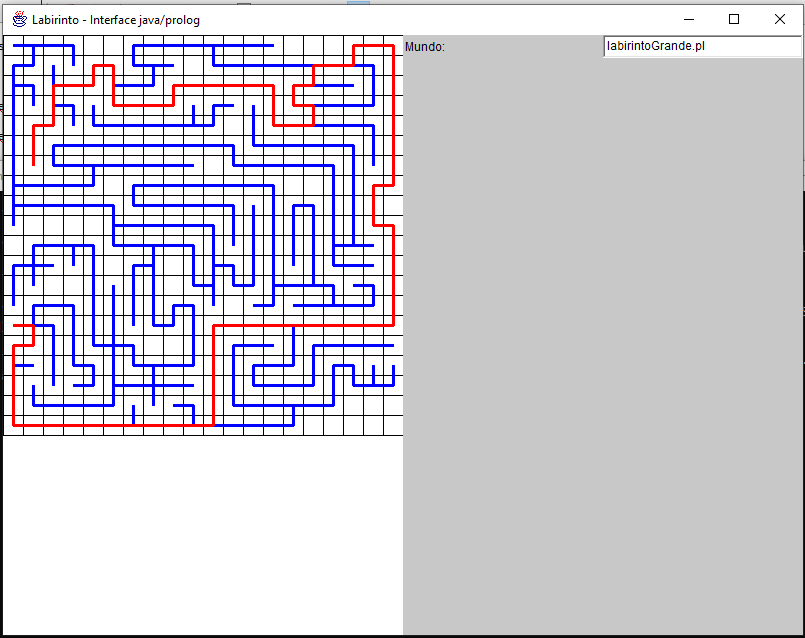
\includegraphics[width=\linewidth]{img/labGrande}
	\caption{Demonstração do cálculo de um caminho num labirinto de grandes dimensões na interface java/prolog}
	\label{fig:ping}
\end{figure}




\end{document}
